\documentclass[apj]{emulateapj}
%\documentclass[manuscript]{aastex} 


\usepackage{graphicx}                        
\usepackage{amsmath}
\usepackage{hyperref}
\usepackage{amsfonts}
\usepackage{amsmath}
\usepackage{amssymb}
\usepackage{amsthm}


%%%%%%%%%%%%%%%0


\begin{document}

\title{EOS notes}
\author{Ana-Maria Piso}

\section{Adiabatic atmospheres}
\label{adiabatic}

%\begin{verbatim}
%Most of the derivations are already in the notes \\
% you wrote,  so it didn't make sense to rewrite \\
%  them. I just wrote the structure equation \\
%   we are trying to solve.
%\end{verbatim}

In the case of an ideal gas, the relation between temperature, density and pressure is given by the ideal gas law:

\begin{equation}
\label{eq:idealgas}
P=\rho \mathcal{R} T,
\end{equation}

\noindent where $\mathcal{R}$ is the specific gas constant. Hydrostatic balance along an adiabat then gives:

\begin{equation}
\label{eq:drdtid}
\frac{dr}{dT}=-\frac{\mathcal{R} r^2}{\nabla_{ad} G M}
\end{equation}

In the case of a non-ideal gas, however, equation (\ref{eq:idealgas}) no longer applies. Further on we derive the structure equations for a non-ideal gas, using $\log P$ (with $P$ the pressure) as the integration variable. We start from hydrostatic equilibrium:

\begin{equation}
\label{eq:hydro}
\frac{dP}{dr}=-\rho g=-\rho \frac{G M}{r^2},
\end{equation}

\noindent which gives 

\begin{equation}
\label{eq:drdp}
\frac{dr}{d\log P} = -\frac{P}{\rho} \frac{r^2}{G m}
\end{equation}

Mass conservation gives:

\begin{equation}
\label{eq:mcons}
\frac{dm}{dr} = 4 \pi r^2 \rho
\end{equation}

From this and equation (\ref{eq:drdp}) we obtain:

\begin{equation}
\label{eq:dmdp}
\frac{dm}{d \log P} = -\frac{4 \pi P}{G m} r^4
\end{equation}

Furthermore, the gravitation and internal energy can be expressed as 

\begin{equation}
\label{eq:degdp}
\frac{d E_g}{d \log P} = 4 \pi P r^3
\end{equation}

\noindent and

\begin{equation}
\label{eq:deidp}
\frac{d E_i}{d \log P} = - \frac{4 \pi u p}{G m} r^4,
\end{equation}

\noindent where $u$ is the internal energy of the gas per unit mass: $u = U/m$.

%we start from the definition of the adiabatic gradient $\nabla_{ad}$, which is valid even in the non-i%deal cases:

%\begin{equation}
%\label{eq:delad1}
%\nabla_{ad}=\frac{\partial \log T}{\partial \log P}=\frac{P}{T}\frac{dT}{dP}
%\end{equation}
%
%It follows that 
%
%\begin{equation}
%\label{eq:dpdt}
%\frac{dP}{dT}=\frac{1}{\nabla_{ad}}\frac{P}{T}
%\end{equation}
%
%Hydrostatic balance gives
%
%\begin{equation}
%\label{eq:hydro}
%\frac{dP}{dr}=-\rho g=-\rho \frac{G M}{r^2}
%\end{equation}
%
%From equations (\ref{eq:dpdt}) and (\ref{eq:hydro}) we thus find:
%
%\begin{equation}
%\label{eq:drdt}
%\frac{dr}{dT}=-\frac{1}{G M} \frac{P}{\rho \nabla_{ad}} \frac{r^2}{T},
%\end{equation}

In the above equations, $\rho$ and $u$ are functions of pressure. In order to solve them we therefore need to know $\rho(P)$ and $u(P)$ for a non-ideal gas. This will be discussed in detail in the next section.

\section{EOS Tables}

We start from the equation of state tables of \cite{saumon95}. These equations of state take into account non ideal interactions, and include physical treatments of dissociation and ionization, caused by both pressure and temperature effects. However, the \cite{saumon95} EOS tables only cover a relatively high range of temperatures and pressures: $2.10 < \log_{10} T(K)<7.06$ and $4<\log_{10}P$(dyn cm$^{-2})<19$. While these ranges may be suitable deep inside the protoplanetary atmosphere, they are no longer valid as we approach the boundary between the convective and radiative regions of the atmosphere. Since the radiative region is approximated as almost isothermal, the temperature at the bottom of this region is close to the disk temperature, which can be as low as a few tens of Kelvin for large semi-major axes. Additionally, the pressure in the disk can be as low as $10^{-1}$ dyn cm$^{-2}$ (\cite{pn05}). As such, for our purposes it is necessary to extend the \cite{saumon95} EOS tables to lower temperature and pressure values.

We choose $\log_{10} T (K)=1$ and$ \log_{10}P$(dyn cm$^{-2})=-4.4$ as our lower boundaries for temperature and pressure, respectively. Our temperature and pressure grid hence becomes: $1 < \log_{10} T(K)<7.06$ and $-4.4<\log_{10}P$(dyn cm$^{-2})<19$. The other quantities in the tables are calculated as follows.

\subsection{Hydrogen}

\label{hydrogen}

For a system of particles, the partition function can be written as the product of all partition functions associated with each type of energy that the system can have:

\begin{equation}
\label{eq:z}
Z=Z_t Z_r Z_v Z_e Z_n,
\end{equation}

\noindent where $Z_t$, $Z_r$, $Z_v$, $Z_e$ and $Z_n$ are the partition functions associated with translation, rotation, vibration, electronic excitation and nuclear excitation, respectively. For hydrogen, electronic and nuclear excitation are only significant at temperatures higher than our region of interest ($\theta_e \approx 12000$ K and $\theta_n >> \theta_e$, where $\theta_e$ and $\theta_n$ are the characteristic temperatures for electronic and nuclear excitation, respectively). As such, we will only take into account the translation, rotation and vibration of the hydrogen molecule:

\begin{equation}
\label{eq:zagain}
Z=Z_t Z_r Z_v
\end{equation} 

The partition function associated with the motion of the center of mass of the molecule is given by (in the classical limit):

\begin{equation}
\label{eq:Zt}
Z_t=(m/2 \beta \pi \hbar^2)^{3/2} V,
\end{equation}

\noindent where $\beta=1/(k T)$ and $V$ is the volume. The rotational partition function is generally written as:

\begin{equation}
\label{eq:Zr}
Z_r=\sum_0^\infty (2 j+1) \exp{\Big[\frac{-j (j+1)\theta_r}{T}\Big]},
\end{equation}

\noindent where $\theta_r$ is the characteristic temperature for rotational motion. In the case of hydrogen, $\theta_r \approx 85$ K. However, molecular hydrogen occurs in two isomeric forms: orthohydrogen, with the proton spins aligned parallel to each other, and parahydrogen, with the proton spins aligned antiparallel. Each isomer has a different rotational partition function; when the spin isomers are in equilibrium, then the partition function can be written as:

\begin{equation}
\label{eq:Zrspin}
Z_r=\sum_0^\infty (2-(-1)^j) (2j+1) \exp{\Big[\frac{-j (j+1) \theta_r}{T}\Big]}
\end{equation}

In our range of temperatures of interest, we found that $Z_r$ converges after about 25 terms in the series.


Finally, the partition function for vibrational motion is given by:

\begin{equation}
\label{eq:Zv}
Z_v=[1-\exp{(\theta_v/T)}]^{-1},
\end{equation}

\noindent where $\theta_v$ is the characteristic temperature for vibrational motion, $\theta_v \approx 6140$ K for hydrogen. 

If the partition function of a system of $N$ particles is known in terms of $(V, T, N)$, the internal energy and entropy of the system can be determined as follows:

\begin{equation}
\label{eq:U}
U_N=k T^2 \Big(\frac{\partial \log{Z}}{\partial T}\Big)_{V, N}
\end{equation}

\begin{equation}
\label{eq:S}
S_N=k \log{Z} + \frac{U_N}{T}
\end{equation}

The energy and entropy per mass will subsequently be:

\begin{equation}
\label{eq:u}
U=\mathcal{R} T^2 \Big(\frac{\partial \log{Z}}{\partial T}\Big)_{V, N}
\end{equation}

\begin{equation}
\label{eq:s}
S=\mathcal{R} \log{Z} + \frac{U}{T}
\end{equation}

Since $Z=Z_t Z_r Z_v$, it is easy to notice that $U=U_t+U_r+U_v$ and $S=S_t+S_r+S_v$, where $U_t$, $U_r$, $U_v$, $S_t$, $S_r$, $S_v$ are the quantities corresponding to the individual translation, rotation and partition functions, respectively.

It can be shown that the entropy per mass due to translational motion can be expressed as:

\begin{equation}
\label{eq:st}
S_t=\mathcal{R} \Big[ \frac{5}{2} \ln{T} - \ln{P} + \ln \Big( \frac{(2 \pi)^{3/2} \mathcal{R}^{5/2} \mu^4}{h^3}\Big) +\frac{5}{2} \Big]
\end{equation}

\noindent with $\mu$ the mean molecular weight. Equation (\ref{eq:st}) is known as the Sackur-Tetrode formula, and it is only applicable to an ideal gas. It can also be easily shown that the internal energy per mass due to translational motion is given by:

\begin{equation}
\label{eq:ut}
U_t=\frac{3}{2} \mathcal{R} T
\end{equation}

Putting all of the above together, we can now evaluate the thermodynamic quantities needed to extend the \cite{saumon95} EOS tables to low temperatures and pressures.

\begin{enumerate}

\item{\textbf{Density.}} In the low temperature, low pressure regime, hydrogen is molecular and behaves like an ideal gas. As such, the density in this region follows the ideal gas law $P=\rho \mathcal{R} T$.
\item{\textbf{Internal energy per mass.}} $U=U_t+U_r+U_v$, where $U_t$ is given by equation (\ref{eq:ut}), and $U_r$, $U_v$ are determined using equations (\ref{eq:u}), (\ref{eq:Zrspin}) and (\ref{eq:Zv}) above.
\item{\textbf{Entropy per unit mass}}. Similarly, $S=S_t+S_r+S_v$, where $S_t$ is given by equation (\ref{eq:st}), and $S_r$, $S_v$ can be determined from equation (\ref{eq:s}) and the calculated expressions for $U_r$ and $U_v$, respectively.
\item{\textbf{Entropy logarithmic derivatives}}. The logarithmic derivatives $S_T$ and $S_P$ are given by:

\begin{equation}
\label{eq:sT}
S_T=\frac{\partial \log{S}}{\partial \log{T}} \Big |_P
\end{equation}

\noindent and

\begin{equation}
\label{eq:sP}
S_T=\frac{\partial \log{S}}{\partial \log{P}} \Big |_T
\end{equation}

We calculate $S_T$ and $S_P$ using the table values for $S$, $T$ and $P$, and a linear central difference formula. 

\item{\textbf{Adiabatic gradient $\nabla_{ad}$}}. The adiabatic gradient is defined as:

\begin{equation}
\label{eq:delad}
\nabla_{ad}=\frac{\partial \log{T}}{\partial \log{P}} \Big |_S = -\frac{S_P}{S_T}
\end{equation}

We evaluate it from the tabulated values for $S_T$ and $S_P$ determined above. Figure 1 shows a contour plot of the adiabatic index for the extended EOS table, while the black lines represent constant entropy curves. The upper right part of the plot ($\log T>2.1$ and $\log P>4$) is based on the \cite{saumon95} EOS table, while the rest of the plot is our extension. We see that the two tables join smoothly for entropy curves between $8.80<\log{S}$(K g$^{-1})<9.07$.

\end{enumerate}

\begin{figure}[h!]
\centering
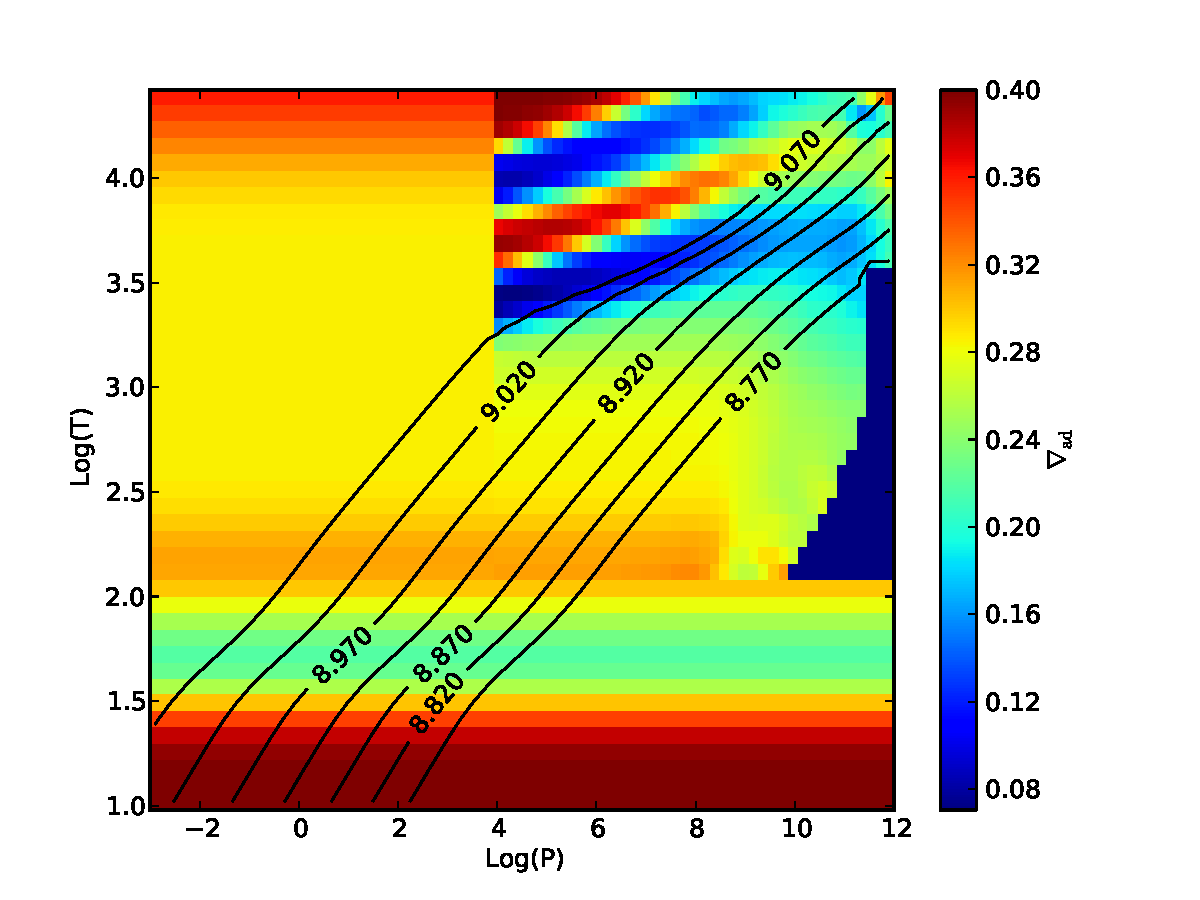
\includegraphics[scale=.5]{../figs/EOS/delad_H_ext}
\caption{$\nabla_{ad}$ contour plot for the hydrogen extended table. The black curves represent constant entropy curves.}
\end{figure}

\subsection{Helium}

We extend the helium EOS tables based on a similar procedure. Since helium is primarily neutral and atomic at low temperatures and pressures, we treat it as an ideal monoatomic gas, and subsequently only take into account the translational components of the necessary thermodynamic quantities (see subsection \ref{hydrogen} above for details). The analogous $\nabla_{ad}$ contour plot for helium can be seen in Figure 2. We notice that, in the case of helium, the original and extended table join smoothly for entropy curves between $8.29<\log{S}$(K g$^{-1})<8.77$.

\begin{figure}[h!]
\centering
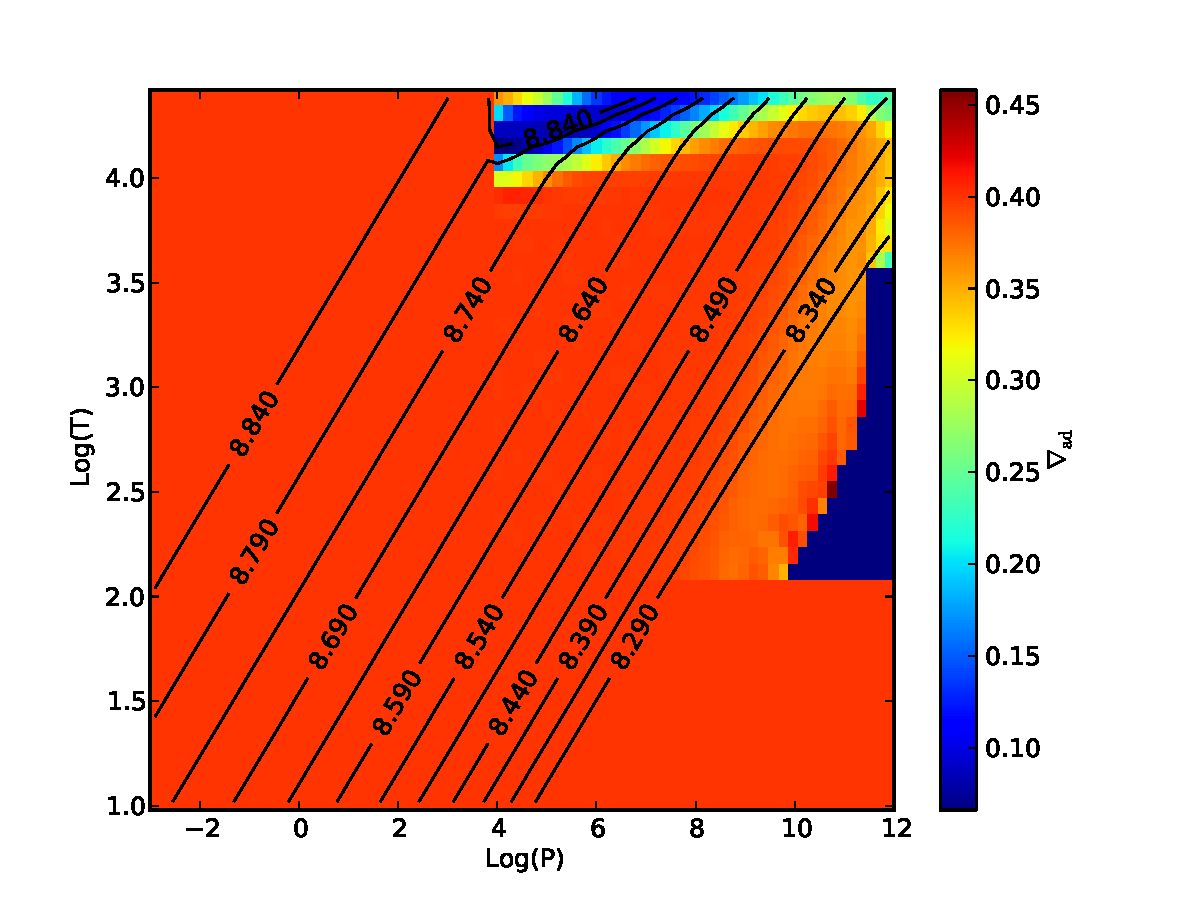
\includegraphics[scale=.5]{../figs/EOS/delad_He_ext}
\caption{$\nabla_{ad}$ contour plot for the helium extended table. The black curves represent constant entropy curves.}
\end{figure}

\subsection{Hydrogen and helium mixtures}

In order to obtain similar EOS tables for hydrogen and helium mixtures, we follow the approach of \cite{saumon95} to calculate the corresponding thermodynamic quantities for the mixture. We denote the helium mass fraction by $Y$. The density of the hydrogen and helium mixture is then given by:

\begin{equation}
\label{eq:rhomixt}
\frac{1}{\rho(P, T)}=\frac{1-Y}{\rho^H(P,T)}+\frac{Y}{\rho^{He}(P,T)}
\end{equation}
 
Similarly, the internal energy per mass of the mixture is given by:

\begin{equation}
\label{eq:umixt}
U(P, T)=(1-Y)U^H(P,T)+Y U^{He}(P,T)
\end{equation}

The entropy per mass can be calculated as:

\begin{equation}
\label{eq:smixt}
S(P,T)=(1-Y)S^H(P,T)+Y S^{He}(P,T)+S_{mix}(P,T),
\end{equation}

\noindent where $S_{mix}$ is given by:

\begin{eqnarray}
\label{eq:smix}
S_{mix}&=&k_B \frac{1-Y}{m_H}\frac{2}{1+X_H+3X_{H_2}} {\ln(1+\beta \gamma)} \nonumber \\
&-&X_e^H \ln(1+\delta)+\beta \gamma [\ln(1+1/(\beta \gamma)) \nonumber \\
&-&X_e^{He} \ln(1+1/\delta)]
\end{eqnarray}

\noindent with 

\begin{equation}
\label{eq:xeH}
X_e^H=\frac{1}{2}(1-X_{H_2}-X_H),
\end{equation}

\begin{equation}
\label{eq:xe}
X_e^{He}=\frac{1}{3}(2-2X_{He}-X_{He^+}),
\end{equation}

\begin{equation}
\label{eq:beta}
\beta=\frac{m_H}{m_{He}} \frac{Y}{1-Y},
\end{equation}

\begin{equation}
\label{eq:gamma}
\gamma=\frac{3}{2}\frac{1+X_H+3+X_{H_2}}{1+2X_{He}+X_{He^+}},
\end{equation}

\begin{equation}
\label{eq:delta}
\delta=\frac{2}{3} \frac{2-2X_{He}-X_{He^+}}{1-X_{H_2}-X_H} \beta \gamma
\end{equation}

The logarithmic derivatives of the entropy (equations(\ref{eq:sT}) and (\ref{eq:sP})) can be evaluated as follows:

\begin{equation}
\label{eq:stmix}
S_T=(1-Y)\frac{S^H}{S}S_T^H+Y \frac{S^{He}}{S}S_T^{He}+\frac{S_{mix}}{S}\frac{\partial \log{S_{mix}}}{\partial \log{T}}\Big |_P,
\end{equation}

\begin{equation}
\label{eq:spmix}
S_T=(1-Y)\frac{S^H}{S}S_P^H+Y \frac{S^{He}}{S}S_P^{He}+\frac{S_{mix}}{S}\frac{\partial \log{S_{mix}}}{\partial \log{P}}\Big |_T,
\end{equation}

The logarithmic derivatives of $S_{mix}$ are calculated from the tabulated values for $S_{mix}$, density and pressure, using a linear central difference formula.

Finally, the adiabatic gradient of the mixture is given by:

\begin{equation}
\label{eq:deladmix}
\nabla_{ad}=-\frac{S_P}{S_T}
\end{equation}

The $\nabla_{ad}$ contour plot analogous to figures 1 and 2 for a hydrogen-helium mixture with $Y=0.3$ can be seen in Figure 3. In the case of the mixture, the original and extended table join smoothly for entropy curves between $8.71<\log{S}$(K g$^{-1})<9.00$.

\begin{figure}[h!]
\centering
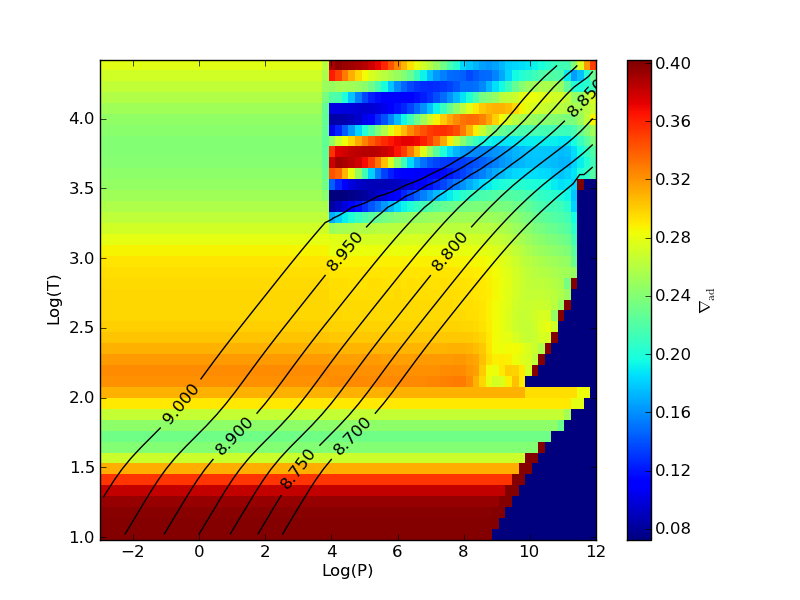
\includegraphics[scale=.5]{../figs/EOS/delad_mixt_ext}
\caption{$\nabla_{ad}$ contour plot for the hydrogen-helium mixture ($Y=0.3$) extended table. The black curves represent constant entropy curves.}
\end{figure}


\section{Numerical atmosphere model}

We are developing a two-layer atmosphere model, with an inner convective region and an outer radiative region that matches onto the protoplanetary disk. One of our main goals is determining the critical core mass for a giant planet to be able to form within the lifetime of the disk (typically of the order of $\sim 10^7$ years), for a variety of disk conditions, and at various distances in the disk. In what follows we approximate the structure of the protoplanet as being spherically symmetric. Figure 4 depicts schematically the structure of our model atmosphere.

\begin{figure}[h!]
\centering
\includegraphics[scale=.33]{../figs/two_layer}
\caption{Schematic depiction of the two-layer model atmosphere: the convective region (of radius $r_{CB}$ and mass $M_{ad}$) and the radiative region (which extends out to the Bondi radius $RB$ and has mass $M_{rad}$) are separated by the radiative-convective boundary.}
\end{figure}

\subsection{Inner Convective Region}

We approximate the inner region as being adiabatic. From section \ref{adiabatic}, the equations that describe the structure of an adiabatic atmosphere are:

\begin{equation}
\label{eq:drdp2}
\frac{dr}{d\log P} = -\frac{P}{\rho} \frac{r^2}{G m}
\end{equation}

\begin{equation}
\label{eq:dmdp2}
\frac{dm}{d \log P} = -\frac{4 \pi P}{G m} r^4
\end{equation}

This is a system of two equations and three unknowns, $r(P)$, $m(P)$ and $\rho(P)$. In order to be able to solve the system we therefore need another relationship between thermodynamic quantities. If the entropy of the system $S$ is assumed to be known, then the density $\rho$ can be uniquely determined as a function of pressure and entropy: $\rho=\rho(P, S)$. 

\subsubsection{Shooting method}

As we will see in the next section, we can determine the temperature and pressure at the radiative-convective boundary from integration of hydrostatic equilibrium in the radiative zone. 





%We denote the radius of the radiative-convective boundary as $r_{CB}$. 

%In what follows we approximate the structure of the protoplanet as being spherically symmetric. Furthermore, we assume hydrostatic equilibrium. As such,
%
%\begin{equation}
%\label{eq:hydroeq}
%\frac{dP}{dr}=-\rho g,
%\end{equation}
%
%\noindent where $g=GM(<r)/r^2$, with $M(<r)$ being the total mass interior to radius $r$.  The mass $M(<r)$ satisfies the equation
%
%\begin{equation}
%\label{eq:m}
%\frac{dM}{dr}=4 \pi r^2 \rho
%\end{equation}
%
%From this and equation (\ref{eq:drdt}) it follows that
%
%\begin{equation}
%\label{eq:dmdT}
%\frac{dM}{dT}=-\frac{4 \pi \rho}{G M} \frac{P}{\rho \nabla_{ad}} \frac{r^4}{T}
%\end{equation}



\bibliographystyle{apj}
\bibliography{refs}


\end{document}